{\color{brown}\textbf{Ejemplo 4}} Un grupo de 64 obreros puede terminar una obra en 15 días. Al cabo de 5 días de trabajo, se les unen obreros de otro grupo, de modo que tardan 5 días menos en terminar la obra.\\
\textbf{¿Cuántos obreros había en el segundo grupo?}\\

Sabemos que 64 obreros terminarían la obra en 15 días. Como luego de los primeros 5 días de trabajo llegaron más obreros, hacemos el siguiente gráfico para representar la situación:
\begin{figure}[H]
    \centering
    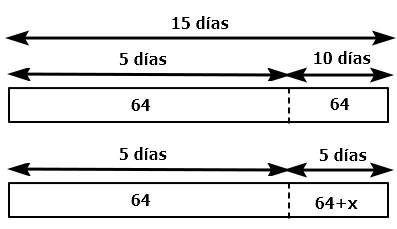
\includegraphics[width=0.4\textwidth]{./Unidad 2/Images/tableS8L103.png}
\end{figure}
Observamos que, en esta situación, a mayor cantidad de obreros, menos días se necesitarán para terminar la obra.\\
\begin{table}[H]
    \centering
    \begin{tabular}{|l|c|l|}
        \hline
        Cantidad de obreros         & 64 & 64+x \\
        \hline
        Cantidad de días de trabajo & 10 & 5    \\
        \hline
    \end{tabular}
\end{table}
Como es una relación inversamente proporcional, planteamos la siguiente relación:
\begin{align*}
    64 \times 10 & = 5 \times (64+x) \\
    640          & = 320 +5x         \\
    5x           & = 320             \\
    x            & = 64
\end{align*}

En el segundo grupo, había 64 obreros más, es decir, un total de 128 obreros.\\